%!TEX program = xelatex
%!TEX root = ./thesis.tex

\section{Experiments on the basic source tasks}

We discuss and compare the methods in solving the basic task "move0" in this section.

As is observed by many studies~\cite{henderson2017matters}, one of the disadvantages with the traditional KL-divergence based is that the performance result could be inconsistent across different runs, due to the agent getting stuck at local minimum. One example is the performance of the ACKTR~\cite{wu2017scalable} method on the "move0" task. An example result is shown in Figure~\ref{fig_acktr_reprod}, where we train the same ACKTR agent on the task "move0" with batch-size 8000, KL-divergence 0.0001 and  20 parallel agents. It appears that one agent gets stuck at the a score below 300 while another continues to improve after reaching the score of 4000. 
\begin{figure}[!htbp]
	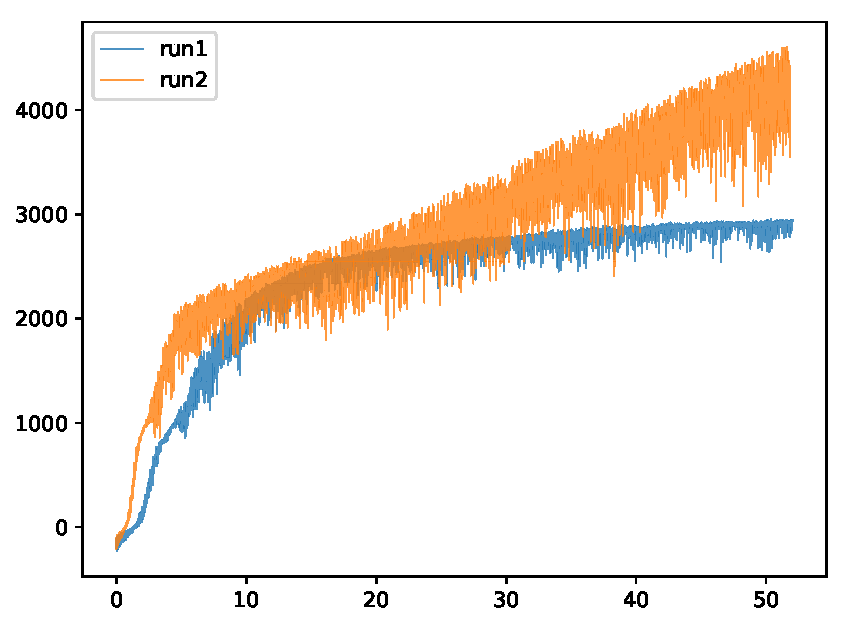
\includegraphics[width=0.7\textwidth]{images/rec_acktr_reprod}
	\centering
	\caption{Inconsistent performance produced by ACKTR agents with the same  parameters but different runs. The vertical axis is the total return averaged over the recent 20 episodes and the horizontal axis is the number of million time-steps}\label{fig_acktr_reprod}
\end{figure}

We observe that the conventional KL-divergence based trust region policy gradient methods in general could get stuck easily at some local minimum before the policy converges to the optimal solution. An experiment showing the performance of the original ACKTR algorithm is shown in Figure~\ref{fig_acktr_mom_tune}. We observe that the agents tend to get stuck around the total return of 3000. The reason might be that while the KL-divergence based trust-region method provides a theoretical guarantee on the monotonic improvement of performance, the agent might converge too early at local minimums and fails to make efficient exploration.
\begin{figure}[!htbp]
	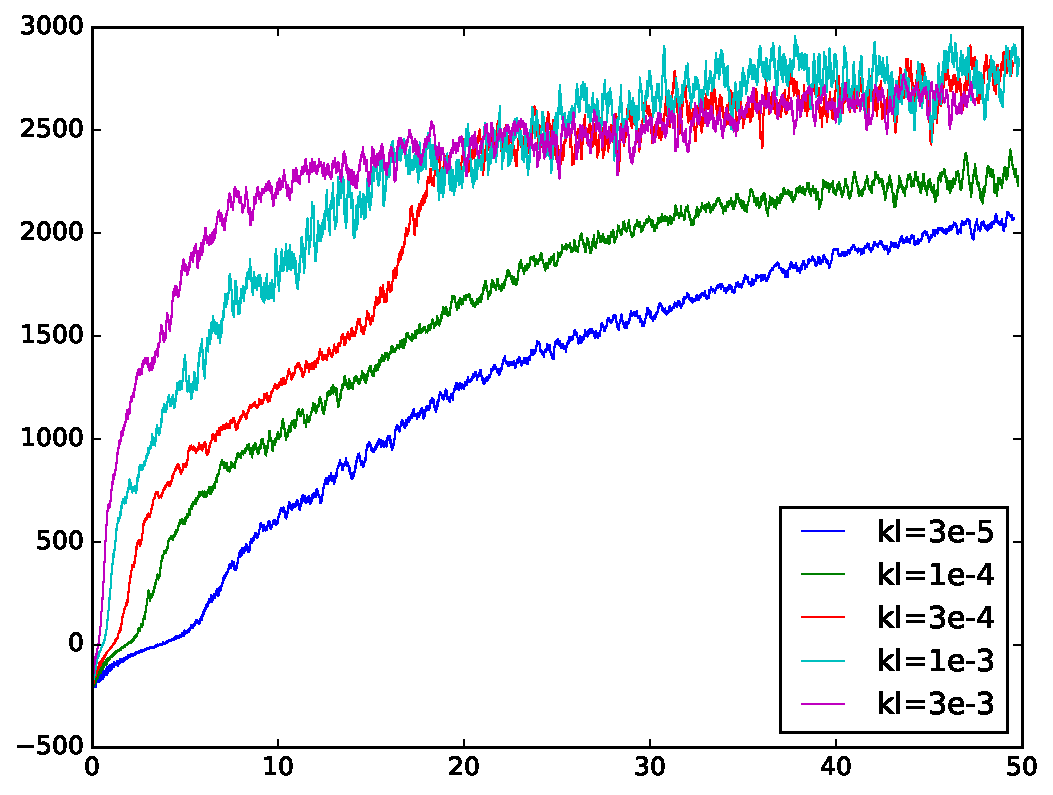
\includegraphics[width=0.7\textwidth]{images/rec_acktr_mom_tune}
	\centering
	\caption{Performance of ACKTR agents with different KL-divergence constraints. All the agents are trained with batch-size 4000 and 20 parallel agents. The vertical axis is the total return averaged over the recent 200 episodes and the horizontal axis is the number of million time-steps}\label{fig_acktr_mom_tune}
\end{figure}

We propose that the proposed W-KTR method is less prune to the local minimum problem on the task "move0". The experiment comparing the performance of W-KTR agents with different parameters is shown in Figure~\ref{fig_wass_const_tune}. We can see that none of the agents get stuck at the local minimum around 3000, and their final performance can reach a total return of 6000. However, the W-KTR agent appears to have a much slower improvement rate before 50 million time-steps.
\begin{figure}[!htbp]
	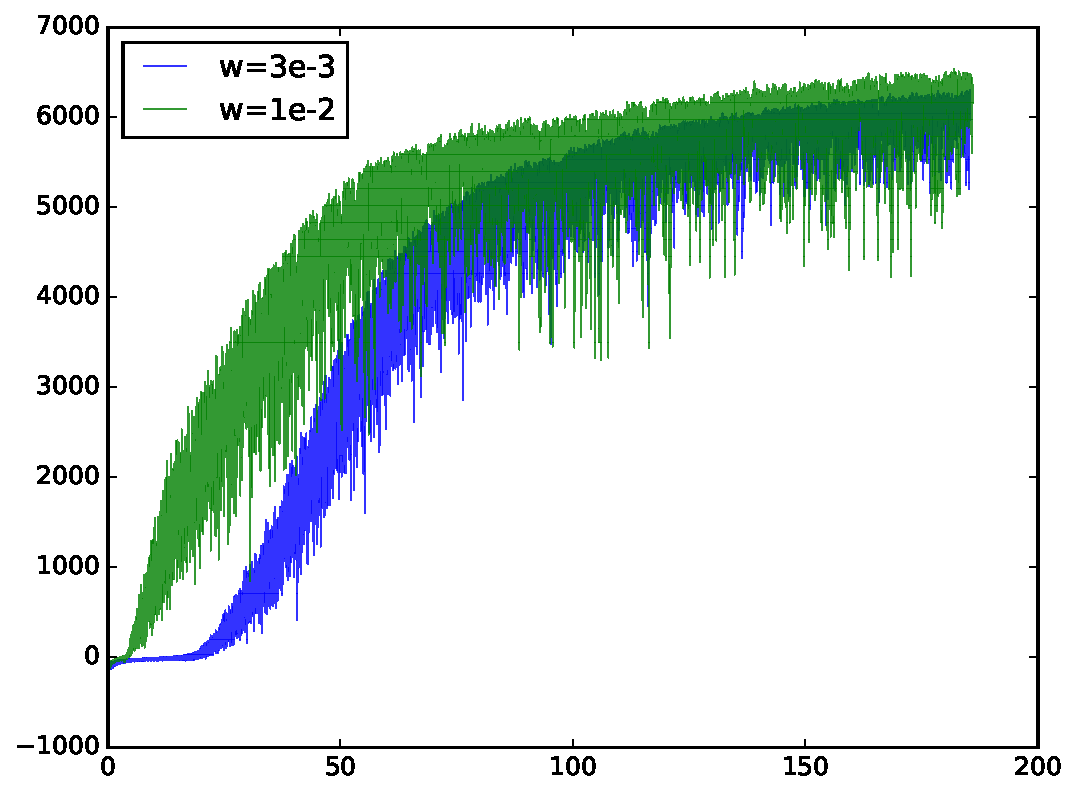
\includegraphics[width=0.7\textwidth]{images/rec_wass_const_tune}
	\centering
	\caption{Performance of W-KTR agents with different W2-metric constraints. All the agents are trained with batch-size 4000 and 20 parallel agents. The vertical axis is the total return averaged over the recent 200 episodes and the horizontal axis is the number of million time-steps}\label{fig_wass_const_tune}
\end{figure}

One proposal to solve the slow initial improvement rate problem of W-KTR method is to apply a decaying Wasserstein constraint at the beginning. The performance of a proposed W-KTR agent with decaying Wasserstein constrainet is shown in Figure~\ref{fig_wass_decay}. The agent can achieve much faster improvement rate in the first 50 million time-steps. The limitation is that there are more hyper-parameters to be tuned in this algorithm.
\begin{figure}[!htbp]
	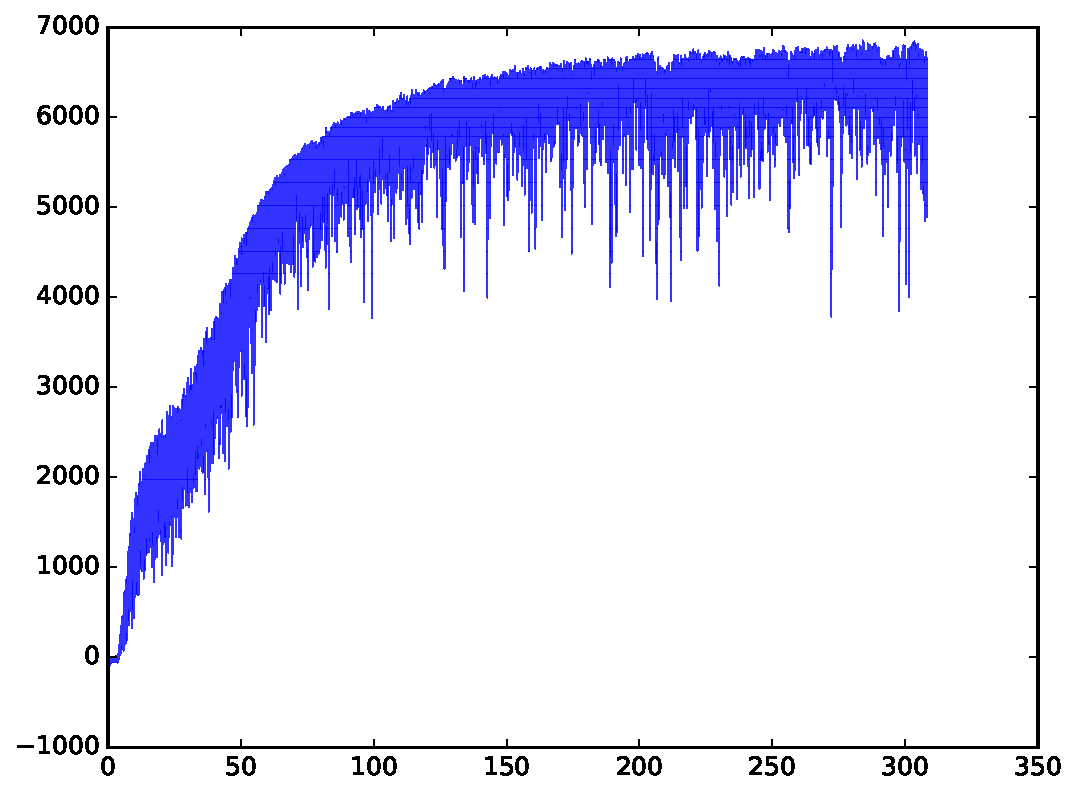
\includegraphics[width=0.7\textwidth]{images/rec_wass_decay}
	\centering
	\caption{Performance of a W-KTR agent with a decaying W2-metric from 0.02 to 0.00003 in the first 15 million time-steps. The agent is trained with batch-size 4000 and 20 parallel agents. The vertical axis is the total return averaged over the recent 200 episodes and the horizontal axis is the number of million time-steps}\label{fig_wass_decay}
\end{figure}

In conclusion, we have verified that the proposed W-KTR method can achieve the state-of-art final performance in the basic "move0" task, and is able to produce consistent final results across different runs.